\usetikzlibrary{calc,decorations.pathreplacing,positioning}%
\begin{tikzpicture}[arrow/.style={->, line width=0.75mm, draw=gray!80}]
    % Titles
    \draw[decorate,decoration={brace, amplitude=0.4em}] (-3.5,0.08) -- (-0.7,0.08) node [midway, above=0.4em] (dataset) {\large \dataset};
    \draw[decorate,decoration={brace, amplitude=0.4em}] (-0.3,0.08) -- (6,0.08) node [midway, above=0.4em] (task) {\large \task};
    \draw[decorate,decoration={brace, amplitude=0.4em}] (6.6,0.08) -- (12,0.08) node [midway, above=0.4em] (score) {\large \score};

    % Subtitles
    \node[font=\bfseries, below left = 0.15cm and 0.85cm of task] (conditions) {\small Conditions};
    \node[font=\bfseries, right = 1.8cm of conditions] (triples) {\small Triples};
    \node[font=\bfseries, right = 2.5 cm of triples]
    (distances) {\small Distances};
    \node[font=\bfseries, right = 1.6 cm of distances] (result) {\small Results};
    
    % Arrows
    \draw[arrow] (-0.7,-2.1) to (-0.3,-2.1);
    \draw[arrow] (1.3,-2.1) to (1.7,-2.1);
    \draw[arrow] (6,-2.1) to (6.4,-2.1);
    \draw[arrow] (8.8,-2.1) to (9.2,-2.1);

    % Dataset
    \node[anchor=north west, below = 0.8cm of dataset] {%
    \scalebox{0.6}{%
    \setlength{\tabcolsep}{5pt}%
    \begin{tabular}{cccc}
    \toprule
    & Fruit & Color & Size \\
    \midrule
    \emoji{red-apple} & Apple & Red & 1 \\
    \emoji{pear} & Pear & Green & 1 \\
    \scalebox{0.7}{\emoji{red-apple}} & Apple & Red &  0.7 \\
    \emoji{green-apple} & Apple & Green & 1 \\
    \scalebox{1.2}{\emoji{green-apple}} & Apple & Green & 1.2 \\
    \multicolumn{4}{c}{$\cdots$} \\
    \bottomrule
    \end{tabular}
    }%
    };

    % Score
    \node[below = 0.05cm of distances] (formula) {\small $d(x,a) < d(x,b)$?};
    \node[below = 0.1cm of formula] {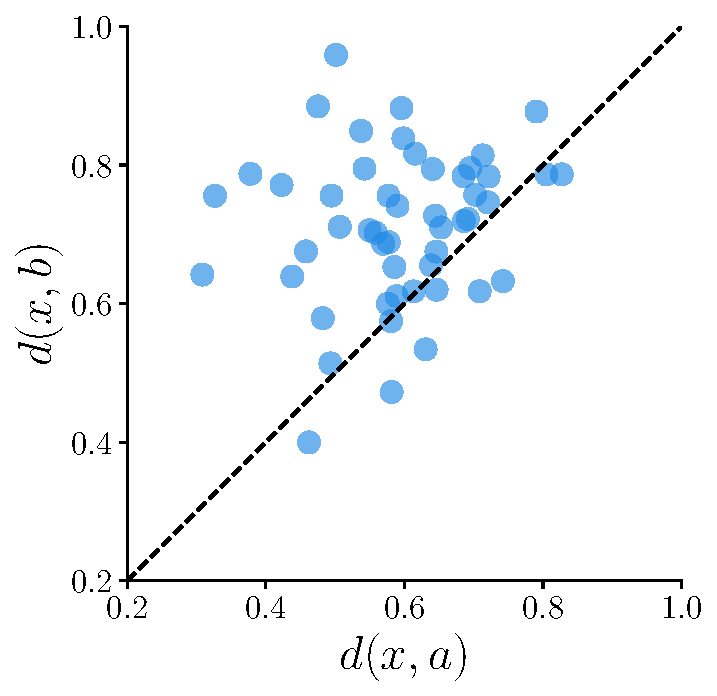
\includegraphics[width=2.25cm]{figures/distances.pdf}};
    \node[below = 0.05cm of result] (confusion) {\small Confusion matrix};
    \node[below = 0.3cm of confusion.north] (matrix){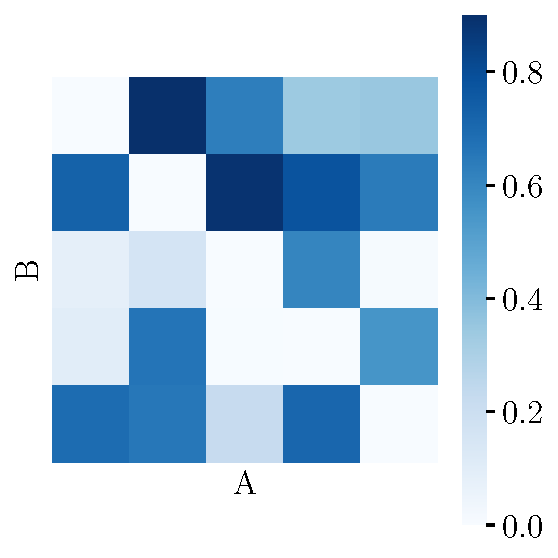
\includegraphics[width=1.9cm]{figures/confusion_matrix.pdf}};
    \node[below = 0.01cm of matrix] {\small $\text{ABX error } = 18.0\%$};

    % Task
    \node[align=center, anchor=west, below = 1.2cm of conditions]{\on fruit\\ \by color};
    \node[anchor=north west, below=0.22cm of triples.center] {%
    \scalebox{0.6}{%
    \setlength{\tabcolsep}{5pt}%
    \begin{tabular}{llcccc}
        \toprule
        & Cell & & $a$ & $b$ & $x$ \\
        \midrule
        \ldelim\{{3}{0cm}  & {%
                            \multirow{3}{*}{%
                            \begin{tabular}{l}
                                $\on_{ax} = \text{Apple}$ \\
                                $\on_{b} = \text{Pear}$ \\
                                $\by_{abx} = \text{Green}$ \\
                            \end{tabular}}}
        & \ldelim\{{3}{0cm} & \scalebox{0.75}{\emoji{green-apple}} & \emoji{pear} & \scalebox{1.2}{\emoji{green-apple}} \\
        & & & \scalebox{1.2}{\emoji{green-apple}} & \emoji{pear} & \scalebox{0.75}{\emoji{green-apple}} \\
        & & & & $\cdots$ \\
        \multicolumn{6}{c}{\large $\cdots$} \\
        \ldelim\{{3}{0cm}  & 
        {\multirow{3}{*}{%
          \begin{tabular}{l}
            $\on_{ax} = \text{Strawberry}$ \\
            $\on_{b} = \text{Apple}$ \\
            $\by_{abx} = \text{Red}$ \\
          \end{tabular}}} & \ldelim\{{3}{0cm}  & \scalebox{1.2}{\emoji{strawberry}} & \scalebox{0.8}{\emoji{red-apple}} & \scalebox{0.8}{\emoji{strawberry}} \\
        & & & \scalebox{0.8}{\emoji{strawberry}} & \scalebox{0.8}{\emoji{red-apple}} & \scalebox{1.2}{\emoji{strawberry}} \\
        & & & & $\cdots$ \\
        \bottomrule
        \end{tabular}%
    }%
    };
\end{tikzpicture}